The PFEM-2 method is a generalization of the Particle Finite Element Method (PFEM) \cite{sergio:pfem} where the particles are not restricted to the mesh nodes. Massless particles are added everywhere in the mesh and the advection is done by transporting the particles. The main benefit is that now the nodes of the mesh do not have to be moved as was the case in \cite{sergio:pfem} saving many re-meshing operations while maintaining the Lagrangian advection. In \cite{sergio:xivs1} Idelsohn et. al. present an integration scheme called {\em eXplicit Integration following the Velocity Streamlines} (X-IVS) which is used to integrate the trajectory of particles in PFEM-2. Using this technique the position of a particle $p$ at time $t^{n+1}$ ($x_p^{n+1})$ is computed using the velocity streamlines at $t^n$:
%
\begin{equation}\label{xivs}
  \begin{cases}
    \vect{x}_p^{n+1}=\vect{x}_p^n+\int_n^{n+1} \vect{u}^n(\vect{x}_p^\tau) d\tau\\
    \hat{\vect{u}}^{n+1}_p=\vect{u}_p^n
  \end{cases}
\end{equation}
%
The expression in Eq. \ref{xivs} is explicit since it only depends on values from time step $t^n$ while it maintains the high order approximation used for the velocity field. This expression is not an exact integration since the integral is evaluated following a pseudo-trajectory of the particles calculated with the velocity streamlines within each time step instead of following the true trajectory. Eq. \ref{xivs} may be integrated analytically or using any standard time integration scheme like explicit Runge-Kutta or using sub-stepping. This new integration proposal provides an efficient strategy to employ time-steps which allow a Courant-Friedrich-Levy (CFL) number larger than one, where:
%
\begin{equation}
  CFL=\frac{|\vect{u}|\Delta t}{\Delta x}
\end{equation}
%
In summary this means that each particle will be able to travel more than one element without compromising the stability of the method.

It is important to remark that the particles carry valuable information from all the states previous to their current location and preserving that information will have a big influence in the final accuracy of the method. That is why instead of interpolating the mesh velocity to the particle the change of the mesh velocity should be applied. So in Eq. \ref{xivs}:
%
\begin{equation}\label{eq:partcor}
  \vect{u}_p^{n}=\vect{u}_p^{n-1}+\sum_{i}N_i(\vect{x}_p^n)(\vect{u}_i^n-\vect{u}_i^{n-1}).
\end{equation}
%
being $N$ the shape function of node $i$ for the host element of particle $p$.
\begin{figure}[htp] 
\centering 
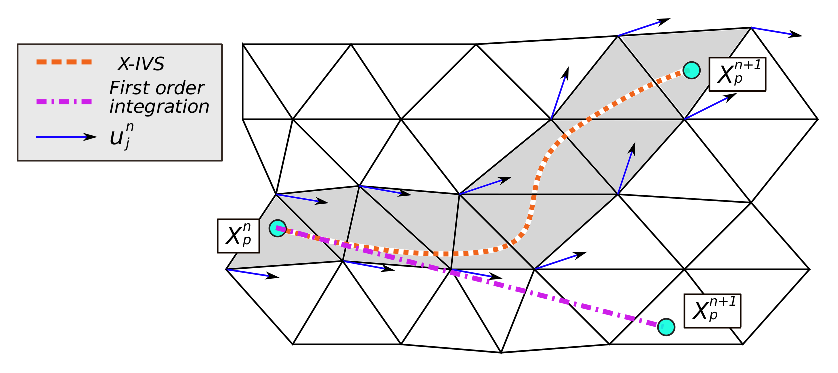
\includegraphics[scale=.6]{./imgs/xivs.eps}
\caption{Comparison of the trajectory of a particle moving from $x_p^n$ to $x_p^{n+1}$ for a given $\Delta t$ using the X-IVS method and a first order integration method. The vectors represent the fluid velocity at time $t^n$.}
\label{fig:xivs}
\end{figure}
%
In Fig. \ref{fig:xivs} the trajectory of a particle is computed using the X-IVS method and it is compared to the trajectory of a first order integration scheme for a $CFL>>1$. 

Once the particles are moved to their new $t^{n+1}$ position the field $\phi$ that they transport (velocity, temperature, level set, etc.) needs to be mapped back to the mesh to perform the FEM analysis. Several approaches have been presented in \cite{gimenez:tesis}. In the current work the Global Least Squares Consistent (GLSC) methodology has been implemented and applied to our test cases. This approach solves a minimization problem where the approximation functions are the same linear shape functions used by the FEM discretization. This results in a global system where the unknowns are the nodal values. The minimization problem will be solved for $\phi$ such that it minimizes a global error function $E_g$ which computes the quadratic difference between the particle states $\phi_p$ at positions $\vect{x}_p$ surrounding a node at position $\vect{x}_j$ and the nodal value $\phi_j$:
%
\begin{equation}\label{eq:minim}
  E_g(\phi_1,\phi_2,...,\phi_j)=\frac{1}{2}\sum_{p=1}^P \biggl(\phi_p-\sum_{j=1}^J\phi_jN_j(\vect{x}_p)\biggr)^2.
\end{equation}
%
To minimize $E_g$ equation \ref{eq:minim} is derived with respect to $\phi_j$ and equaled to zero leading to the system of $J$ unknowns:
%
\begin{equation}\label{eq:mapptom}
  \vect{M}\vect{\phi}=\vect{f}
\end{equation}
%
where $J$ is the total number of nodes in the mesh, $\vect{M}_{ij}=\sum_pN_i(\vect{x}_p)N_j(\vect{x}_p)$ is a consistent mass matrix, $\vect{\phi}$ are the unknown nodal values and $\vect{f}_i=\sum_pN_i(\vect{x}_p)\phi_p$.

A step by step summary of the final algorithm for solving Navier-Stokes using fractional step and PFEM-2 is explained in Algorithm \ref{algo:pfem2}.
%
\begin{algorithm}[H]
%\floatname{algorithm}{Fractional Step with PFEM-2}
\floatname{algorithm}{Algorithm}
%\renewcommand{\thealgorithm}{}
\caption{Summary of the steps needed for solving Navier-Stokes using fractional steps and PFEM-2.}
\label{algo:pfem2}
\begin{algorithmic}[1]
\STATE Compute the convection moving particles along streamlines (X-IVS)(Eq. \ref{xivs}).
\STATE Map particle velocities to mesh (Eq. \ref{eq:mapptom}).
\STATE Solve the system of Eq. \ref{eq:masamat}-\ref{eq:matunm2} with $\beta=0$.
\STATE Correct velocity on particles (Eq. \ref{eq:partcor}).
\STATE Reseed particles if necessary.
\STATE Remove particles if allowed.
\end{algorithmic}
\end{algorithm} 
%
Another aspect of PFEM-2 which is more widely discussed in \cite{gimenez-difusion} is that of particle inventory. Essentially it is the question of when, where and how to add or remove particles. In the present implementation particles are seeded into all the elements at initialization. There is a constant amount of particles per element at the beginning of a run. The number of initial particles can change for different problems. In this work all elements are seeded with twelve initial particles in $3-d$ and nine in $2-d$. Since the objective of this paper is to evaluate the accuracy of PFEM-2 and compare it to that of FEM and experimental results then no strategy has been used to remove particles for the results presented later. The idea is to use PFEM-2 to it's full accuracy capacity and removing particles is associated to a lose of accuracy by introducing numerical diffusion. Particles are added to the simulation to maintain a minimum amount of particles per element. This is a difference compared to \cite{gimenez-difusion} where the metric used to add particles is associated to the node. This will obviously decrease the computational performance of the simulation since the amount of particles will increase. The implementation relies on a robust parallel implementation to account for the increased demand of memory and CPU due to the increased number of particle. More on this subject will be explained in the next section. As an example to illustrate this issue a simple problem considering the flow past a $2-d$ cylinder is used (see Fig. \ref{fig:cyl_def}). It is better to use a $2-d$ model for illustrative purposes. In Fig. \ref{fig:cyl_evol} the initial configuration ``A'' is compared to an advanced configuration ``B''. Initially all elements have the same amount of particles and the distribution is homogeneous. As the flow evolves particles agglomerate increasing the overall amount of particles in the domain. Finally figure \ref{fig:cyl_npart} shows a curve with the number of particles as a function of time. Note how the number of particles increase rapidly at the beginning of the simulation and then reaches a pseudo-steady state amount. The objective of future implementations will be to attempt to maintain a constant number of particles while preserving the accuracy of the method. There is more about the particle inventory implications for parallel implementations in the next section.
%
\begin{figure}[htp] 
\centering 
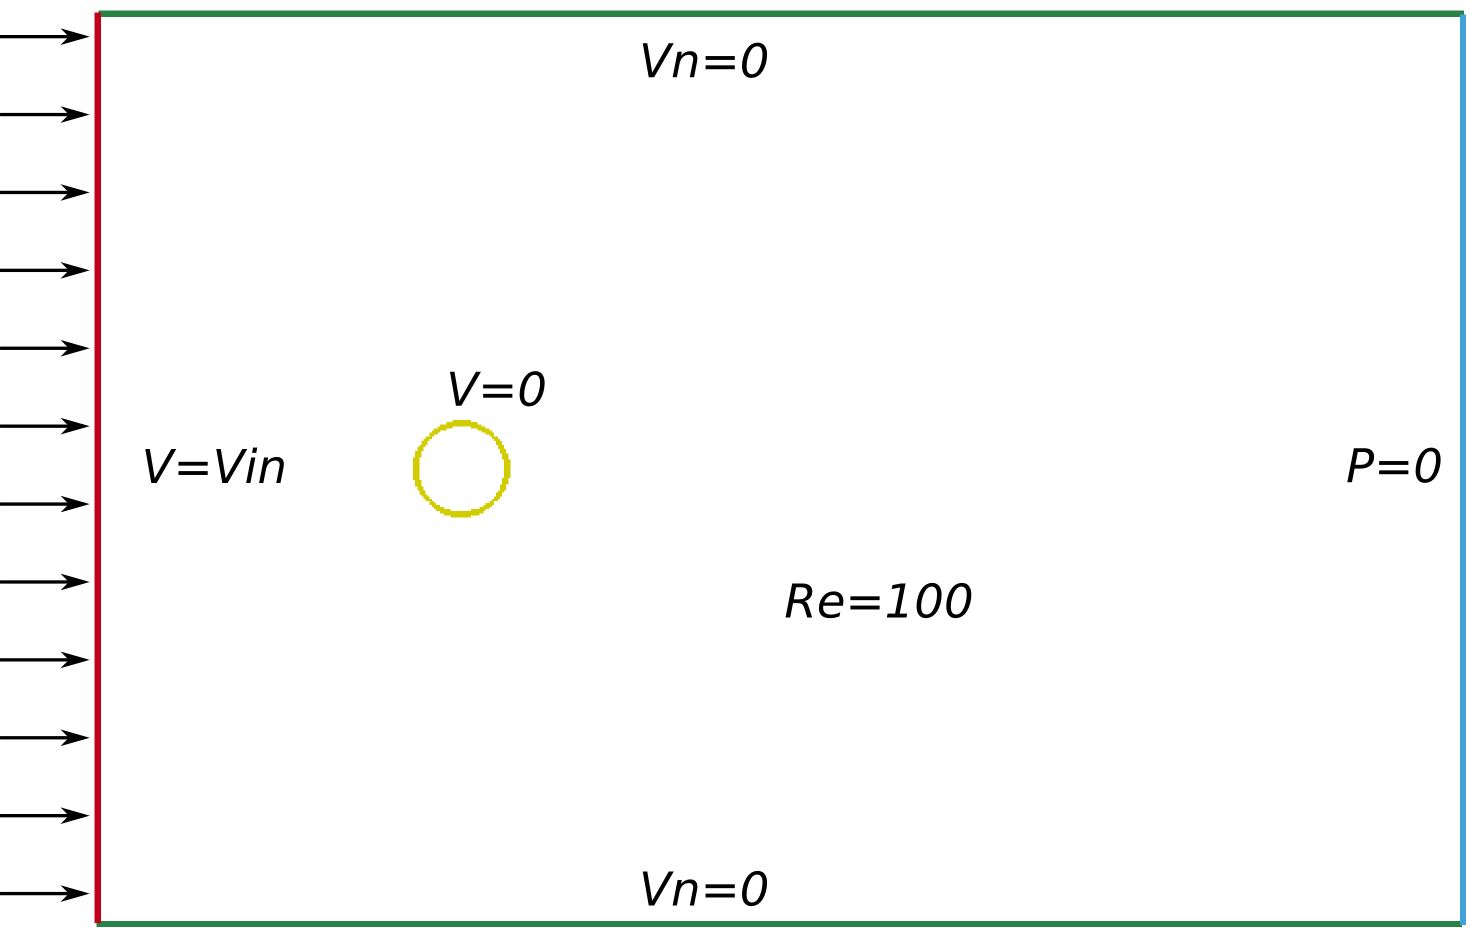
\includegraphics[scale=.5]{./imgs/cyl_def.png}
\caption{Problem definition for the $2-d$ cylinder problem and boundary conditions.}
\label{fig:cyl_def}
\end{figure}
%
\begin{figure}[htp]
\centering 
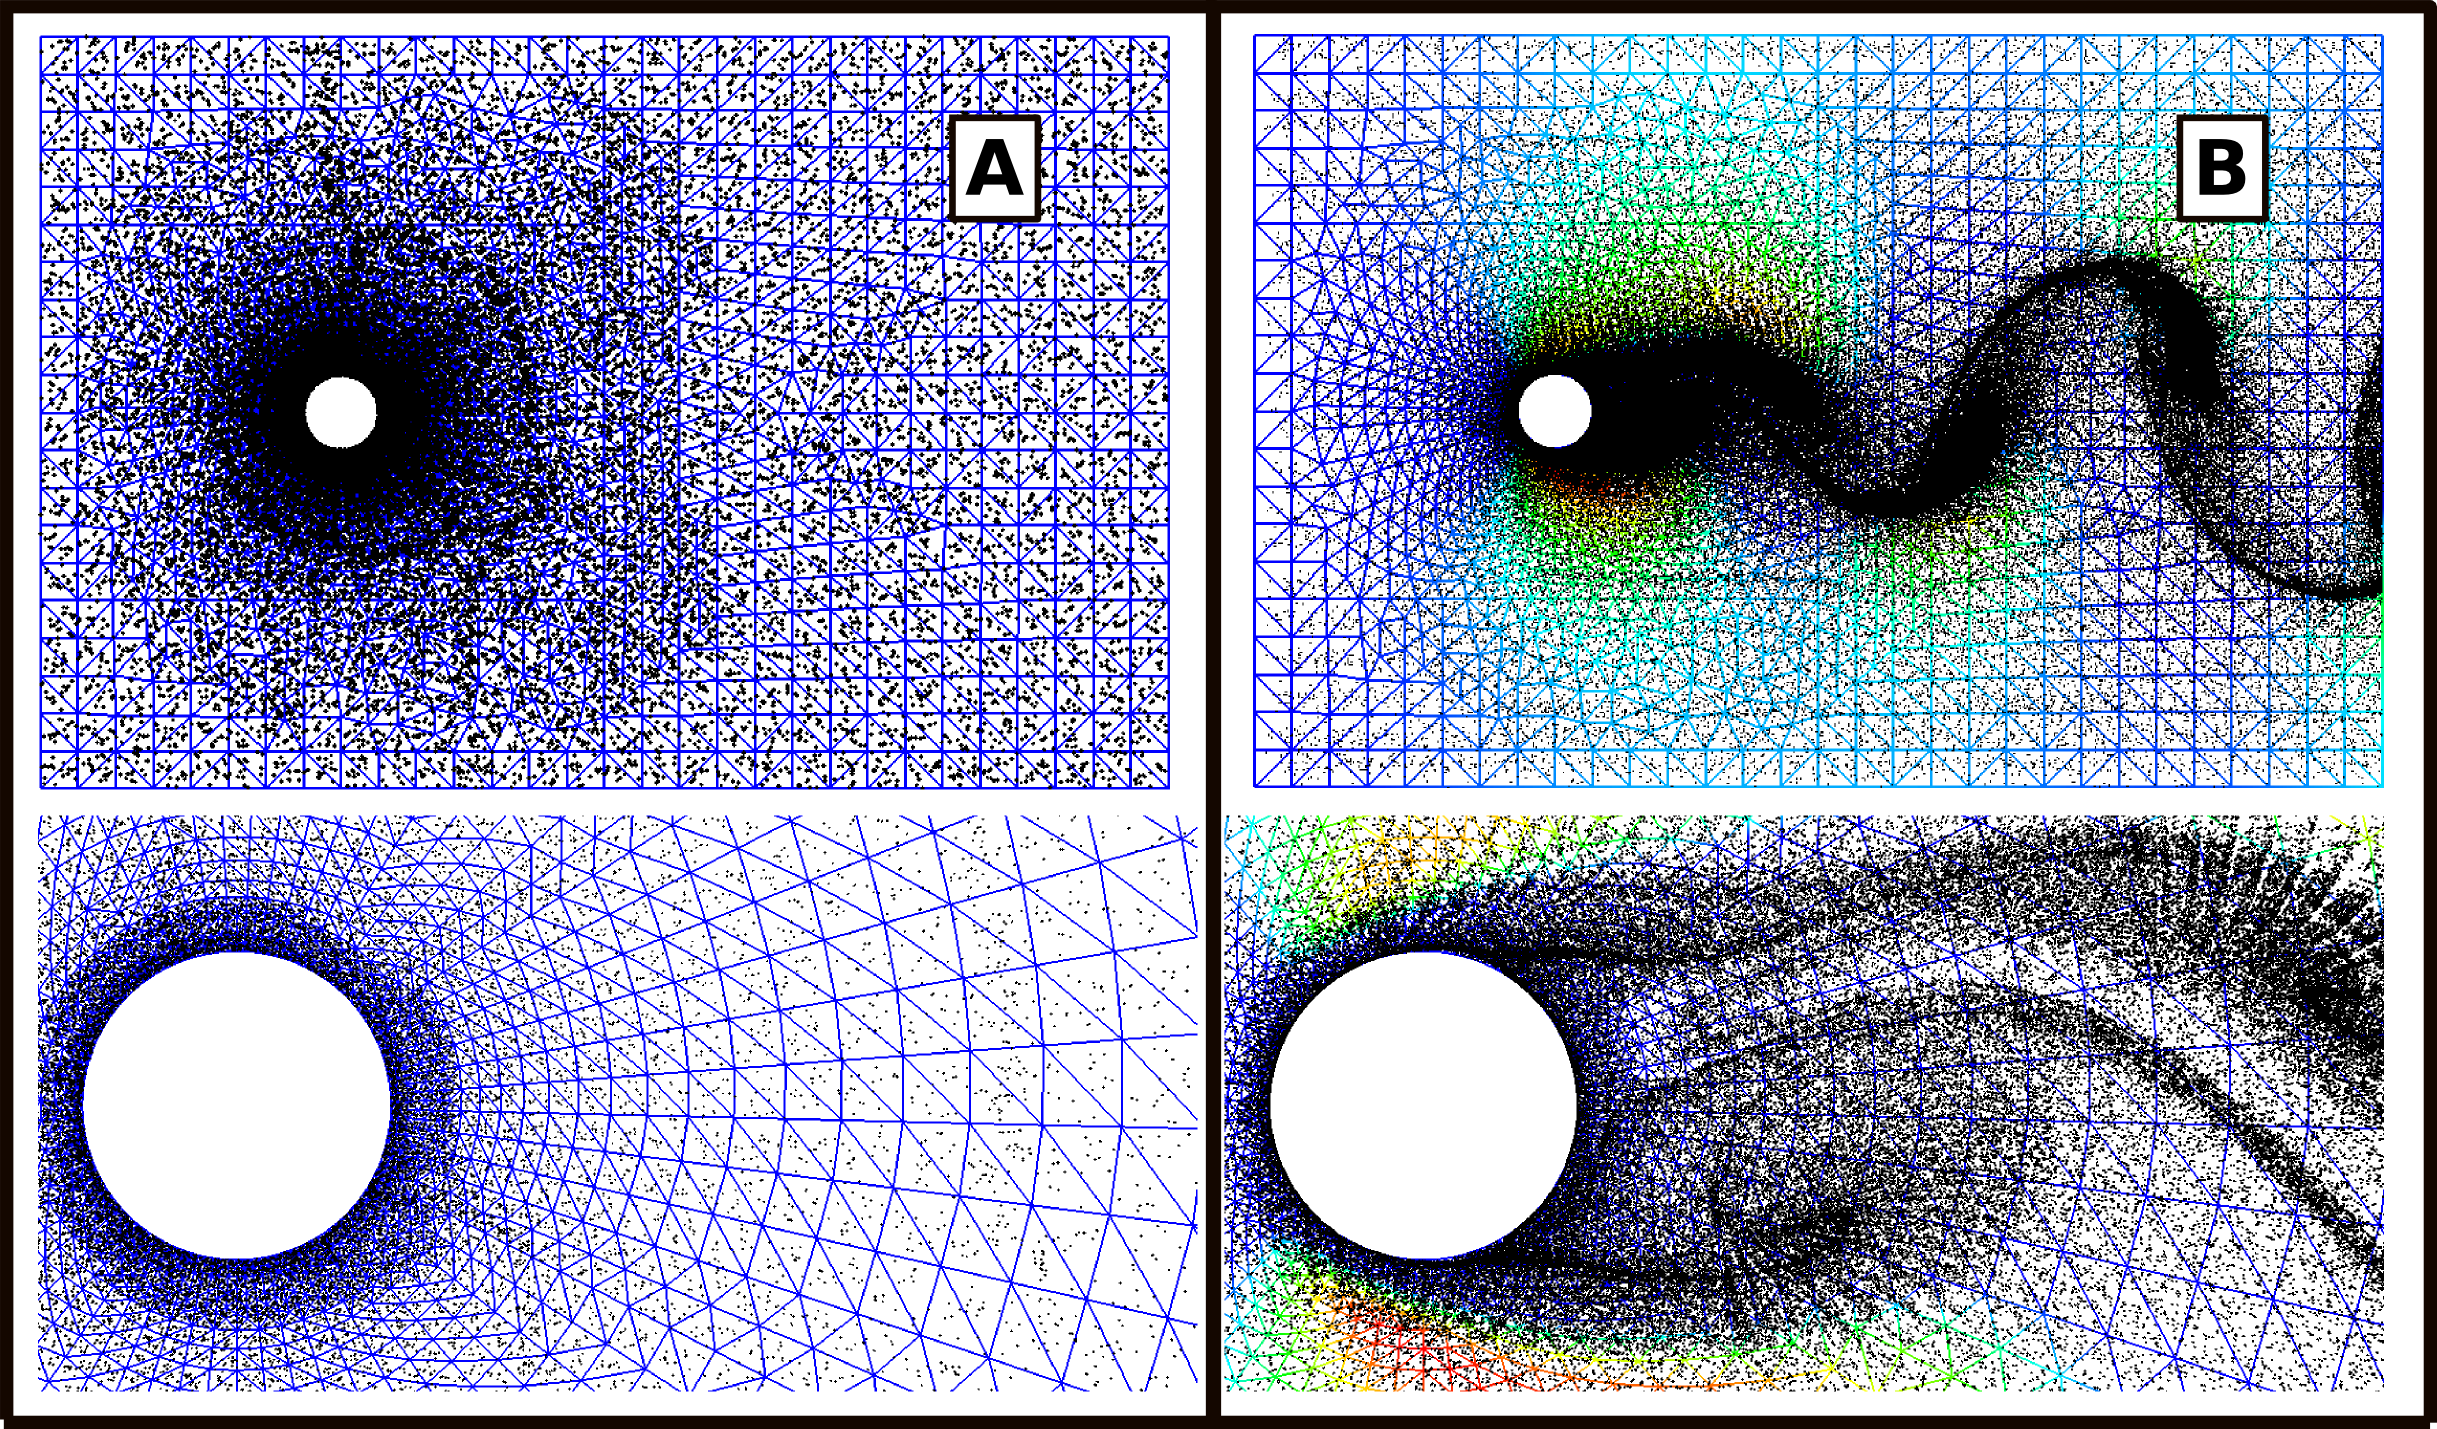
\includegraphics[scale=.4]{./imgs/cyl_parts.png}
\caption{Evolution of particle position and number of particles for the $2-d$ cylinder problem. A) Initial configuration and B) advanced particle configuration.}
\label{fig:cyl_evol}
\end{figure}
%
\begin{figure}[htp] 
\centering 
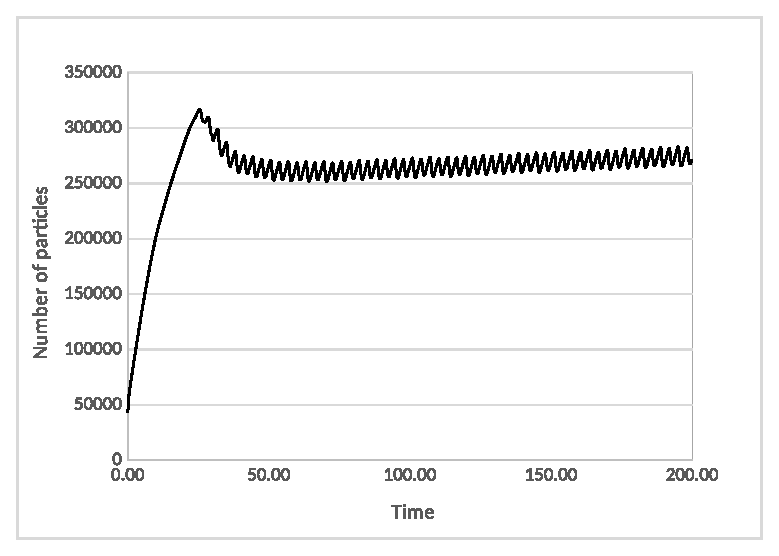
\includegraphics[scale=.6]{./imgs/npart_cyl_excel.eps}
\caption{Number of particles as a function of a non-dimensional time for the cylinder problem. Observe how to particle number increase rapidly and then they reach a pseudo-steady state amount.}
\label{fig:cyl_npart}
\end{figure}
